%===============================================================================
\section{Example: Luminosity function estimation}
\label{sec:lum_func}

The CUDAHM distribution contains some example code implementing basic hierarchical models, such as the normal-normal model, and a realistically complicated astrophysical example handling regression with classical measurement error, with nonlinear models (the interstellar dust problem described above).

As a somewhat more complicated application of CUDAHM, we here consider luminosity function estimation, a parametric conditional density estimation problem arising across many areas of astronomy.
We highlight this example, both because of its ubiquity across astronomy, and to illustrate the generality of CUDAHM.
We describe luminosity function estimation for a model including, not only measurement error, but also \emph{selection effects}.
The selection effects make the joint distribution structure more complicated than the conditional density estimation DAG shown in Fig.~\ref{fig:DAGs}; in particular, there are two plates (corresponding to detected and undetected objects).
However, the likelihood function can be manipulated to have a conditional dependence structure similar to that of a single-plate DAG, allowing straightforward implementation of the model using CUDAHM.

%-------------------------------------------------------------------------------
\subsection{Astronomical background}
\label{sec:LF-astro}

%\enote{Introductory content here was moved from Janos's intro.}

The fundamental observables for localized astronomical sources include position (both direction on the celestial sphere, and distance, $r$, in some chosen coordinate system), and apparent brightness, quantified in terms of flux, $F$.
Astronomers use these observables to study demographic properties of many classes of sources, including stars and galaxies of various types, minor planets (such as asteroids), and explosive transients (gamma-ray bursts, supernovae).
For concreteness, here we focus on observations of nearby galaxies, for which distance may be measured by using spectroscopy to find the \emph{redshift}, $z$, of spectral lines (i.e., their fractional shift in wavelength from laboratory values).
Due to the cosmological expansion, for relatively nearby galaxies, distance is proportional to redshift,
\begin{equation}
r = \frac{cz}{H_0},
\label{eq:H0}
\end{equation}
where $c$ denotes the speed of light, and $H_0$ is Hubble's constant, measuring the current expansion rate of the universe, with $H_0 \approx 70$~km~s$^{-1}$~Mpc$^{-1}$ (with Mpc denoting megaparsecs).
$H_0$ is measured with a precision of several percent, and spectroscopic redshifts for nearby galaxies can be measured to sub-percent precision.
For simplicity, here we consider distances to be precisely measured, via spectroscopic redshifts.
Often, astronomers use redshift directly as a proxy for distance.

A fundamental intrinsic characteristic of a source is its \emph{luminosity} (emitted power), $L$, a measure of its intrinsic (vs.\ apparent) brightness.
For nearby galaxies (i.e., for distances where space is very nearly Euclidean), the inverse-square law relates $L$ to the observables $F$ and $r$:
\begin{equation}
F=\frac{L}{4\pi r^2}.
\label{eq:inv-sqr}
\end{equation}
The \emph{luminosity function}, $\lfunc(L, d)$, describes the distribution of intrinsic brightness for a population at a specified distance (or redshift).
It is typically defined as the intensity function for a point process, i.e., as specifying the expected number of galaxies per unit volume at distance $d$, per unit luminosity interval.
If we denote the spatial number density of galaxies at distance $r$ by $n(r)$, then $n(r) = \int dL\, \lfunc(L, r)$.
The \emph{luminosity PDF} for galaxies at distance $r$ is then
\begin{equation}
\lpdf(L,r) = \frac{\lfunc(L, r)}{n(r)}.
\label{eq:lpdf}
\end{equation}
Note that $\lfunc(L,r)$ and $\lpdf(L,r)$ specify \emph{conditional} distributions, i.e., distributions for $L$ at a given $r$.%
\footnote{Authors vary on the definition of the luminosity function, many defining it as done here, and others using ``luminosity function'' to denote what we here call the luminosity PDF.}
Using (\ref{eq:inv-sqr}), the \emph{flux PDF} for galaxies at distance $r$, denoted $\rho(F,r)$, can be found by a change of variables from $L$ to $F$, giving
\begin{equation}\label{eq:rho-f}
\rho(F,r) = 4\pi r^2 f(4\pi r^2 F, r).
\end{equation}

The galaxy luminosity function carries valuable information about the formation and evolution of galaxies, therefore it is an important target of inquiry in astronomy.
CUDAHM can address parametric luminosity function inference; we denote the luminosity function parameters by $\theta$.
For simplicity we here focus on a homogeneous population, so that the distance dependence may be ignored, but it is important in many applications.
The following development is straightforward to generalize to account for models with distance dependence in the luminosity function.

%-------------------------------------------------------------------------------
\subsection{Parametric luminosity function models}
\label{sec:lfmodels}

For most cosmic populations, including galaxies, the luminosity function falls very steeply with increasing luminosity.
The canonical starting point for parametric modeling of luminosity distributions is the \emph{Schecter function},
\begin{equation}
\lfunc(L;\theta) =
  \frac{A}{L_*} \left(\frac{L}{L_*}\right)^{\beta} e^{-L/L_*},
\label{eq:schecter}
\end{equation}
where the parameters $\theta = (L_*,\beta, A)$ comprise a luminosity scale, $L_*$, a power law index, $\beta$, and an amplitude, $A$.%
\footnote{There are varying conventions for parameterizing the amplitude of the Schecter function.
In this parameterization, $A$ has units of space density.
In similar parameterizations, $A$ is often denoted $\lfunc_*$, although it neither has the units of $\lfunc$, nor is it equal to $\lfunc(L_*)$, as the symbol might misleadingly suggest.}
The form of the Schecter function would seem to imply a luminosity distribution that is a gamma distribution (with shape parameter $\alpha = \beta - 1$).
However, the observed samples of many populations follow Eq.~\ref{eq:schecter} with $\beta$ in the interval $(-2,-1)$, in which case the integral of $\lfunc(L;\theta)$ over $L$ is infinite, and the luminosity distribution is formally improper (with $\alpha$ outside of the allowed range for the gamma distribution).
Low-luminosity sources are unobservable (due to noise and background, discussed below), so in practice the \emph{observable} luminosity function is truncated at low luminosities, and the impropriety is often ignored.
But the actual luminosity function must rise less quickly with decreasing $L$ (corresponding to $\beta$ becoming larger than $-1$) or be cut off at low luminosities (corresponding to there being a minimum galaxy size).

%\enote{Perhaps move some of the following details to an appendix?}

For some populations, an increase in the power law index (i.e., flattening of the slope) is in fact observed at low luminosities.
For example, the stellar initial mass function (related to the stellar luminosity function, and fit with similar models) has a low-mass (low-luminosity) index that increases by $\approx 1$ (REF).
Motivated by such observations, and to keep the luminosity distribution proper, we here adopt a ``break-by-one'' (BB1) generalization of the Schecter function, with $\lfunc \propto L^{\beta+1}$ at low luminosities, and thus integrable for $\beta > -2$.
Specifically, the BB1 model has a luminosity distribution with three parameters: a mid-luminosity power law index, $\beta$, and two parameters defining the mid-luminosity range, $(l, u)$, with $l < u$ and  $u$ playing the role of $L_*$ in the Schecter function, and the power law index smoothly breaking to $\beta+1$ as $L$ decreases below $l$.
The BB1 luminosity PDF has following functional form:
\begin{equation}
\label{eq:lumPDF} 
\lpdf(L ; \theta) = 
  \frac{C(\beta,u,l)}{u}\left(1-e^{-L/l}\right) \left(\frac{L}{u}\right)^{\beta} e^{-L/u},
\end{equation}
where the normalization constant $C(\theta)$ is
\begin{equation}
\label{eq:normLumPDF} 
C(\beta,u,l) =
  \begin{cases} \dfrac{1}{\Gamma(\beta+1)\cdot\left(1-\frac{1}{\left(1+\frac{u}{l}\right)^{\beta+1}}\right)} 
    & \quad \text{if } \beta > -2\text{ and }\beta \ne -1; \\
 \dfrac{1}{\log\left(1+\frac{u}{l}\right)} & \quad \text{if } \beta=-1.
  \end{cases}
\end{equation} 
Note that as $l\rightarrow 0$, the BB1 distribution becomes a gamma distribution (if $\beta > -1$).
%Also, in our computational implementation, the condition $\beta=-1$ of the first case is $-1.001<\beta<-0.999$.
We designed the BB1 distribution to have smooth power law break behavior at low $L$, yet also have an analytical normalization constant;
it is proper for $\beta > -2$.
It can also be sampled from using a straightforward modification of a widely-used algorithm for sampling from the gamma distribution (REF).
These properties make it useful for simulation experiments.

We define a BB1 luminosity function by multiplying the BB1 luminosity distribution by the galaxy spatial number density, which is simply a constant, $n$, for a homogeneous population.
Fig.~\ref{fig:lumfunc} shows an example BB1 luminosity function, with $\beta = 1.5$, and $(l,u) = (5\times 10^{10}, 5\times 10^{12})$ in dimensionless units; it is plotted both with $\log$-linear axes, and with $\log$-$\log$ axes, where the varying power law behavior is evident.
The local power law index corresponds to the slope, $G(L)$, in $\log$-$\log$ space, defined by
\begin{equation}
	G(L) \equiv \frac{\dd\log{\lpdf}}{\dd\log{L}} = \frac{L}{\lpdf} \frac{\dd \lpdf}{\dd L} = g(L) + \beta - \frac{L}{u},
\end{equation}
with
\begin{equation}
	g(L) = \frac{L}{l}\cdot\frac{1}{e^{L/l} - 1}.
\end{equation}
Evidently, $g(L) \rightarrow 0$ for $L \gg l$ and $g(L) \rightarrow 1$ for $L \ll l$.
Thus the logarithmic slope, $G(L)$, corresponds to an exponential cutoff at large $L$, and at small $L$, a slope of $\beta + 1$.
When $u\gg l$, so there is a range where $L\gg l$ but $L\ll u$, the logarithmic slope is $\approx \beta$ in that range.

\begin{figure}
	\begin{subfigure}[c]{0.45\textwidth}
		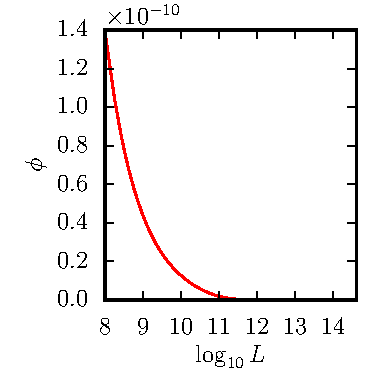
\includegraphics{fig/lumfunc_loglin}
		\caption{}
	\end{subfigure}
	\begin{subfigure}[c]{0.45\textwidth}
		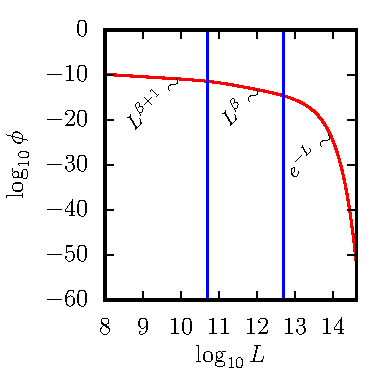
\includegraphics{fig/lumfunc_loglog}
		\caption{}
	\end{subfigure}
	\caption{Example BB1 truncated broken power law PDF, on a log-linear scale (a) and on log-log scale (b), with parameters $(u,l) = (5\times 10^{10}, 5\times 10^{12})$ in dimensionless units, and $\beta = -1.5$.
	In Panel~b the blue verticals show the lower limit $l$ and upper limit $u$ of the region where the power law slope is $\approx\beta$.}
	\label{fig:lumfunc}
\end{figure}

Finally, the BB1 cumulative distribution function is 
\begin{equation}
\label{eq:lumCDF} 
\lcdf(L ; \theta) = 
  C(\theta)
  \left[ \Gamma(\beta + 1) - \gamma\left(\beta + 1, L/u\right) - \frac{\Gamma(\beta + 1)-\gamma\left(\beta + 1, L\cdot\left(\frac{1}{u}+\frac{1}{l}\right)\right)}{\left(1 + \frac{u}{l}\right)^{\beta + 1}} \right],
\end{equation}
where $\Gamma(\cdot)$ and $\gamma(\cdot, \cdot)$ denote the gamma function and the upper incomplete gamma function, respectively.

%-------------------------------------------------------------------------------
\subsection{Modeling survey selection effects and measurement error}
\label{sec:slxn+err}

Astronomers estimate luminosity functions and other astronomical distributions using data compiled in \emph{survey catalogs}: tables of estimates (including uncertainties) of object properties, accompanied by a description of selection criteria for the survey that produced the catalog.
Catalogs are derived data products; they summarize information in more complex and voluminous raw datasets, such as large collections of images or time series.
The nature of astronomical catalog data makes their analysis differ in some respects from analyses of survey data familiar in the statistical survey sampling literature.

Flux measurements are affected by measurement error that is often dominated by Poisson fluctuations in the photon counting rate, including fluctuations from astrophysical and instrumental backgrounds.
The measurement error thus approximately scales with the square root of the flux, and is fractionally greater at low flux than at high flux.
At low fluxes, photons from the backgrounds can produce false source detections.
To prevent this, surveys adopt detection criteria to strongly mitigate against false detections.
A simple, representative criterion is to accept sources only if the estimated flux is $\nu$ times the flux uncertainty, with $\nu \approx 5$ so that the probability for false detection is low even for large catalogs (i.e., there is strong control of the family-wise error rate).

Detection criteria introduce \emph{selection effects} into catalogs.
Most obviously, faint sources (low luminosity sources, or distant high luminosity sources) are excluded; the observable luminosity function is a thinned version of the actual luminosity function.
In addition, \emph{measurement error} more subtly but significantly distorts the shape of the observable distribution, a phenomenon well known in the density deconvolution literature, and also recognized in the astronomical literature, where it is sometimes called \emph{Eddington bias}, in reference to early discussions of the distortion by Eddington and Jeffreys (REFS).
They noted that an object with a measured flux of $\hat F$ is more likely to be an object with a true flux $F < \hat F$ than one with $F > \hat F$, even when measurement errors have a symmetric distribution, because dim sources are more numerous than bright sources in most astronomical settings.
Selection effects can exacerbate the distortion in the vicinity of a flux threshold, with measurement error and the falling flux distribution conspiring to scatter more below-threshold sources into the observed sample than above-threshold sources out of it, a component of what astronomers call \emph{Malmquist bias} \citep{binney1998galactic} (although the term is used inconsistently).
Hierarchical modeling can automatically account for such thinning and distortion, in a manner that adapts to the shape of the luminosity function; this is a major motivation for its increasing popularity in astrostatistics.

We have developed a framework for modeling astronomical survey data using \emph{thinned latent marked point process models}.
Measurement error is handled in a hierarchical Bayesian manner, by introducing latent member property parameters, with catalog estimates understood as describing member likelihood functions for the properties.
We model the population distribution of the latent member properties using marked point processes.
We model selection effects through thinning of the latent point process.
We outline the framework here as it applies to luminosity function estimation and similar problems, in contexts where a marked Poisson point process is an appropriate model for the latent member properties. 

A somewhat subtle aspect of the problem is the tie between measurement error and selection effects.
In astronomical surveys, the raw data are scanned to find candidate objects.
For candidates that pass detection criteria, the data are used to estimate source properties.
The same underlying data are used both for selection (detection) and measurement; these tasks are not independent, as is assumed in many statistical survey methods.
Ignoring the dependence can corrupt inferences (REF?).

Object detection is typically implemented via a scanning procedure.
For example, for image data, a fixed aperture may be scanned over the image; a specified algorithm determines if an object is present, e.g., by comparing the estimated flux in the aperture to a threshold value (set by background and noise estimates), or by fitting an image model to the data in the aperture and comparing the fitted amplitude to a threshold.
For time series data, a window may be scanned over the time series, with an object detected if the estimated flux is above a threshold.
If an object is detected, its properties are estimated, e.g., by a likelihood or weighted least squares calculation, with estimation results summarized in the catalog.

Fig.~\ref{fig:ScanMark} illustrates the framework and its relationship to catalog construction.
We split the object property parameter space into scan and mark components.
The scan component corresponds to the dimensions over which the detection scan operates; 
%(e.g., two-dimensional position for image data, or arrival time for time series data).
the mark component corresponds to the remaining dimensions.
For our galaxy luminosity function example, the scan component is the two-dimensional position of the galaxy image on the detector (corresponding to its direction on the sky), and the mark component is the galaxy luminosity and distance, or equivalently, flux and distance (in a more complex case, the mark component might include color and morphological parameters).
In the figure, the dots (red) indicate the true properties of seven galaxies; the blue contours depict likelihood functions for the properties, based on noisy image data.
The gray region at the bottom is bounded above by the position-dependent detection threshold; an object is detected only if its best-fit (maximum likelihood) flux is above the threshold.
Here two of the seven galaxies are not detected.

\begin{figure}
\begin{center}
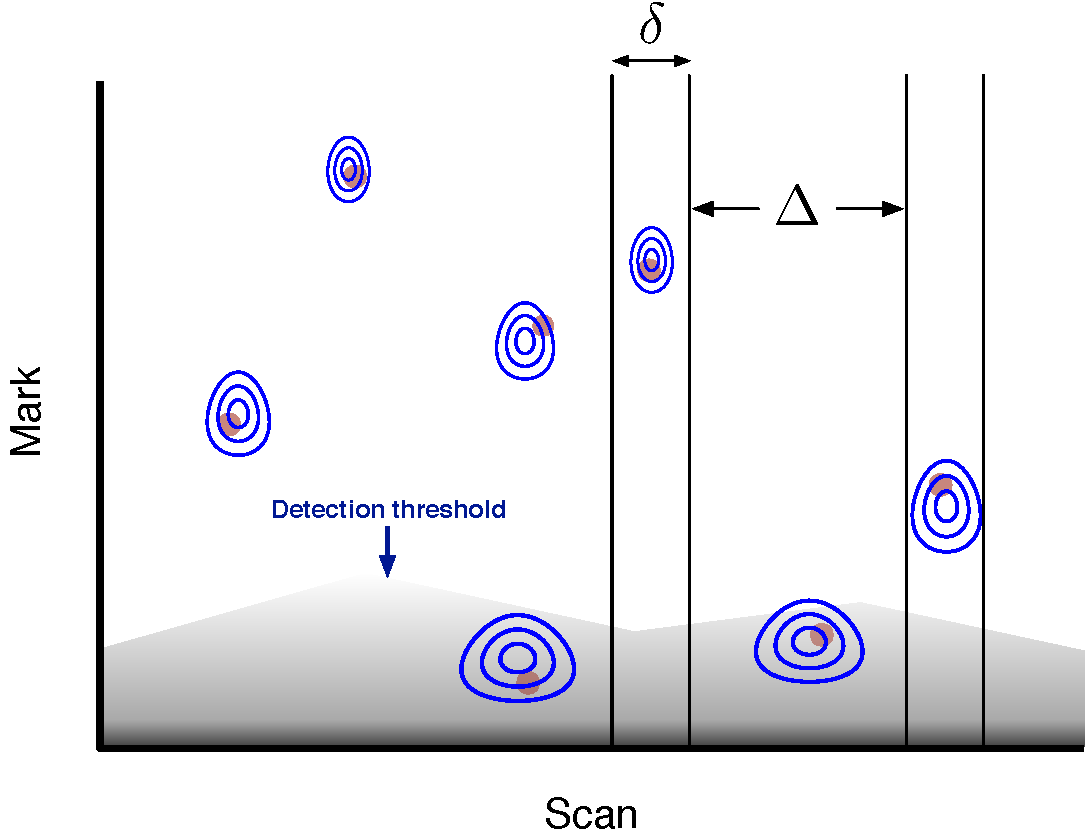
\includegraphics[width=.8\textwidth]{fig/ScanMarkPtProcess-Thin+Err}
\end{center}
\caption{Depiction of thinned latent marked point process model for catalog data produced by an astronomical survey.
Object properties are split into a scanned subset and a mark subset.
Dots (red) show latent (true) values for an object's properties.
Contours (blue) depict member likelihood functions from analysis of the raw survey data; catalogs provide summaries of these for detected objects.
Gray region at bottom depicts the non-detection region; candidates with estimated mark values below a varying threshold are rejected.
$\delta$ and $\Delta$ denote sizes of detection and nondetection intervals.}
\label{fig:ScanMark}
\end{figure}











%-------------------------------------------------------------------------------
\subsection{Hierarchical model for luminosity function inference}
\label{sec:hm}



%-------------------------------------------------------------------------------
\subsection{Simulation setup}
\label{sec:simsetup}

In case of real measurements the distance of the objects is known from redshift observations.
In our simplified case we assume these distance measurements to be without error.
To compile the simulated data set, we assume a spherically symmetric, homogeneous distribution of galaxies and generate the random distances $r_i$ accordingly.
We use the inverse-square law
\begin{equation}
F_i = \frac{L_i}{4 \pi r_i^2}.
\end{equation}
The observational noise $E$ of the flux $F$ is modelled as Gaussian with zero mean and a standard deviation of
\begin{equation}
\sigma(F)=\sqrt{\sigma_{0}^2+(0.01F)^2}.
\label{eq:error}
\end{equation}
The flux limit of the telescope is the constant $T$ and $C$ will denote the event when an object is detected, i.e. the noisy flux is above the threshold: $D > T$.
When generating the random sample, the luminosity is limited between $10 \leq \log_{10}{L} \leq 14$ which implies the distance limit
\begin{equation}
r_\textnormal{max} = \sqrt{\frac{L_\textnormal{max}}{4 \pi T}}.
\end{equation}

As it was discussed above in Sec.~\ref{sec:intro}, the spatial distribution of galaxies is considered homogeneous, hence the density function becomes \begin{equation}\label{eq:dist_dens_func} \delta(r)= \begin{cases} \dfrac{3r^{2}}{r_{\max}^{3}} & \quad \text{if } 0\leq r\leq r_{\max}\\ 0 & \quad \text{otherwise} \end{cases} \end{equation} and the cumulative distribution function: \begin{align}\label{eq:dist_cum_func} \Delta(r)= \begin{cases} 0 & \quad \text{if } r<0\\ \dfrac{r^{3}}{r_{\max}^{3}} & \quad \text{if } 0\leq r\leq r_{\max}\\ 1 & \quad \text{if } r\geq r_{\max} \end{cases} \end{align}


%-------------------------------------------------------------------------------
\subsection{Choice of prior}

Now we consider the choice of prior for the population parameters.
For $\beta$, we adopt a prior that is flat with respect to the angle in $\log$-$\log$ space.
This choice has the virtue of not putting a lot of prior probability on the steep slope range, which a flat prior on $\beta$ would do.
Denoting the angle by $\varphi$, if we adopt a prior PDF of $h(\varphi)$ on $\varphi$, the prior on $\beta = \tan\varphi$ is
\begin{equation}
	p(\beta) = \frac{h(\varphi)}{1 + \beta^2}.
\end{equation}
For a flat $\varphi$ prior between two cut-offs $\varphi_L$ and $\varphi_U$,
\begin{equation}
	p(\beta) = \frac{1}{\varphi_U - \varphi_L} \cdot \frac{1}{1 + \beta^2}.
\end{equation}
This is a truncated Cauchy distribution.
The Break-By-1 distribution requires $\beta > -2$, corresponding to $\varphi_L = -1.107$.
If we require Eq.~\ref{eq:lumPDF} to be decreasing, the upper limit becomes $\beta < 0$, corresponding to $\varphi_U = 0$.
Thus, the prior on $\beta$ is
\begin{equation}
p(\beta) = \frac{0.903}{1 + \beta^2} \quad \quad \quad \textrm{for} -2 < \beta < 0.
\end{equation}
For the upper scale we use a log-flat prior, a conventional choice for a scale parameter that must be positive, even though this will be improper on both sides, we can ignore the impropriety and the normalizing constant since the likelihood function will make the posterior proper.
A prior flat in $\log{u}$ corresponds to $p(u) \propto \frac{1}{u}$.
The lower scale $l$ must be below the upper scale $u$, which we can ensure by using a prior factored as $p(l, u) = p(u) p(l \assm u)$ and taking $p(l \assm u)$ to vanish for $l \geq u$.
A log-flat prior also seems appealing for $l$ but the data (i.e. luminosity measurements) do not probe the distribution down to zero due to the flux limit of the telescope, we could not have a proper prior without introduction a lower cut-off.
Instead, we simply use a flat prior on $l$.
Hence, the overall prior will be \begin{equation}\label{eq:popParsPriorPDF} p(\beta, l, u) \propto \frac{l}{u \cdot (1 + \beta^2)} \quad\quad\quad \textrm{for} -2 < \beta < 0, l < u.
\end{equation}

%-------------------------------------------------------------------------------
\subsection{Working with the Flux Limit}
\label{sec:sel_effect}

In order to implement the hierarchical Bayesian model outlined above, we have to calculate the probability distribution of functions of the characteristics and the population parameters, cf. Eq.~\ref{eq:chi_sampling}~and~\ref{eq:theta_sampling}.
In our particular case the characteristics are the noiseless fluxes $F_i$ (or real intrinsic luminosities $L_i$, as distances are known exactly).
The population parameters are $\beta$, $u$ and $l$.
The measurements in our case are the noisy fluxes $D_i$ and the $C$ selection effect is the event when $D > T$, i.e. the observed flux surpasses the limit $T$ of the telescope.
Modeling assumptions $M$ involves selection effect, known distances and the standard deviation of observational noise.
Eq.~\ref{eq:chi_sampling} becomes
\begin{align}
& p(F_{i} | M, \theta, D_{i})=p(F_{i} | C, \sigma(F_{i}), r_{i}, \theta, D_{i})\\
& =\frac{p(C | D_{i}, F_{i}, \sigma(F_{i}), r_{i}, \theta)\cdot p(D_{i} | F_{i}, r_{i}, \sigma(F_{i}), \theta)\cdot p(F_{i} | r_{i}, \sigma(F_{i}), \theta)\cdot p(r_{i}, \sigma(F_{i}), \theta)}{p(C, \sigma(F_{i}), r_{i}, \theta, D_{i})}\\
& \propto \underbrace{p(C | D_{i}, F_{i}, \sigma(F_{i}), r_{i}, \theta)}_\text{$=1$}\cdot p(D_{i} | F_{i}, r_{i}, \sigma(F_{i}), \theta)\cdot p(F_{i} | r_{i}, \sigma(F_{i}), \theta)\label{eq:chi_est_one_prob}\\
& =p(D_{i} | F_{i}, \sigma(F_{i}))\cdot p(F_{i} | r_{i}, \theta)
\end{align}
The term with the brace equals to 1 since all galaxies must surpass the flux limit in order to be in the sample.
At the same time,
\begin{align}
\label{eq:chi_given_dist_theta} p(F_{i} | r_{i}, \theta) = \frac{d}{dF_{i}}\clfunc(F_{i}4\pi r_{i}^{2} ; \theta) = \lfunc(F_{i}4\pi r_{i}^{2} ; \theta)\cdot 4\pi r_{i}^{2}.
\end{align}

To take the selection effect of the flux limit into account, we have to calculate the probability of measuring a galaxy with a given luminosity and distance above the flux limit.
By assuming Gaussian noise, as we already did in Sec.~\ref{sec:bb1truncpl}, the sought probability becomes
\begin{align}
p(C | L, r) &= p(C | F) = \Pr(D>T | F)\\
&= \Pr(F+E>T)\\
&=\Pr(\underbrace{F + E}_\text{$\sim \mathcal{N}\left(F,\sigma(F)\right)$} > T)\\
&=\frac{1}{2}\left( 1 + \erf\left( \frac{F - T}{\sqrt{2}\sigma(F)} \right) \right)\\
&=:\zeta(F ; T,\sigma_{0})
\label{eq:pclr}
\end{align}

We now calculate the probability of \textit{any} galaxy being observed above the flux limit.
Here we make the assumptions that $L$, $r$ and the population parameters $\theta$ are independent.
From Eq.~\ref{eq:pclr}, if follows that
\begin{align}
\mu(\theta):=p(C|\theta)
&=\int_{-\infty}^{\infty} \int_{-\infty}^{\infty} p(C, L, r | \theta)\, \mathrm{d}L \, \mathrm{d}r \\
&=\int_{-\infty}^{\infty} \int_{-\infty}^{\infty} \frac{p(C, L, r, \theta)}{p(\theta)} \, \mathrm{d}L \, \mathrm{d}r \\
&=\int_{-\infty}^{\infty} \int_{-\infty}^{\infty} \frac{p(C | L, r, \theta)\cdot p(L | r, \theta)\cdot p(r | \theta)\cdot p(\theta)}{p(\theta)}\, \mathrm{d}L \, \mathrm{d}r \\
&=\int_{-\infty}^{\infty} \int_{-\infty}^{\infty} p(C | L, r)\cdot p(L | \theta)\cdot p(r)\, \mathrm{d}L \, \mathrm{d}r \\
&=\int_{-\infty}^{\infty} \int_{-\infty}^{\infty} \zeta\left(\frac{L}{4\pi r^2},T,\sigma_{0}\right)\cdot\lfunc(L|\theta)\cdot \delta(r)\, \mathrm{d}L \, \mathrm{d}r.
\label{eq:mu}
\end{align}

The probability of a galaxy with true luminosity at a given distance surpassing the flux limit can be calculated as
\begin{align}
\lfunc^T(L ; r, \theta):&=p(L | C, r, \theta)
=\frac{p(L, C, r, \theta)}{p(C, r, \theta)} \\
&=\frac{p(C | L, r, \theta)\cdot p(L | r, \theta) \cdot p(r, \theta)}{p(C | r, \theta)\cdot p(r, \theta)} \\
&=\frac{p(C | L, r)\cdot p(L | \theta)}{p(C | \theta)} \\
&=\frac{\zeta\left(\frac{L}{4\pi r^2} ; T,\sigma_{0}\right)\cdot \lfunc(L | \theta)}{\mu(\theta)}.
\label{eq:lum_dens_func_with_seleff}
\end{align}
Using Eq.~\ref{eq:chi_given_dist_theta} and (the deduction of) Eq.~\ref{eq:lum_dens_func_with_seleff}, we obtain \begin{align}\label{eq:chi_dens_func_with_seleff} p(F_{i} | C, r_{i}, \theta) = \frac{\zeta(F_{i} ; T,\sigma_{0})\cdot \lfunc(4\pi r_{i}^2F_{i} ; \theta)\cdot 4\pi r_{i}^2}{\mu(\theta)}=\lfunc^{T}(F_{i} ; r_{i}, \theta)\cdot 4\pi r_{i}^{2}.
\end{align} Eq.~\ref{eq:chi_dens_func_with_seleff} is the flux density function with the selection effect taken into account.
In Fig.~\ref{fig:lumfunc_histo} we plot the logarithm of $\lfunc(L ; \theta)$ and $\lfunc^{T}(L ; r, \theta)$ to illustrate the difference introduced by the selection effect.

\begin{figure}
\begin{center}
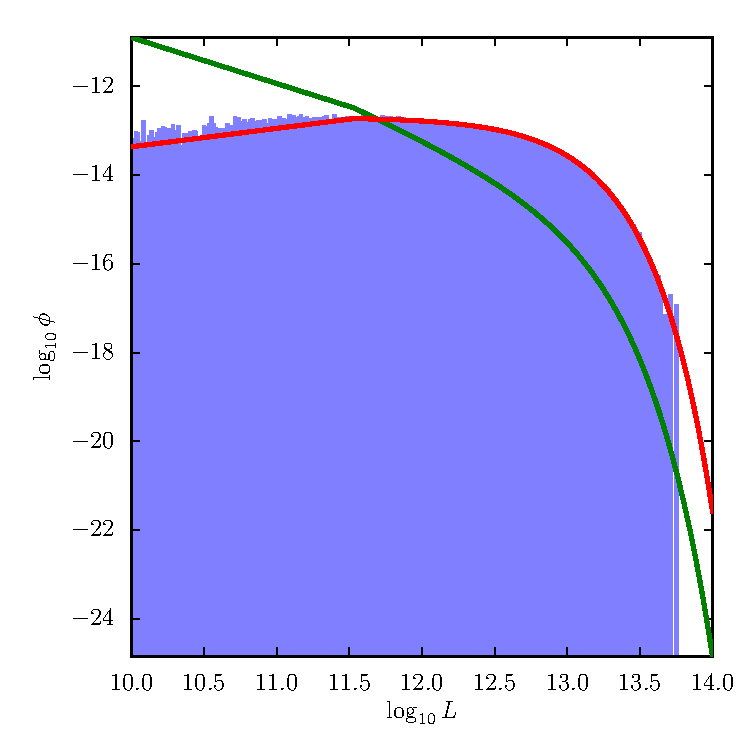
\includegraphics{{fig/lumfunc_histo}}
\end{center}
\caption{The luminosity function $\lfunc(L ; \theta)$ (green curve) and the luminosity distribution of galaxies affected by the Malmquist bias $\lfunc^{T}(L ; r, \theta)$ (red curve). We generated 100{,}000 galaxies with noisy flux (blue histogram). In case of the random sample, the limiting flux was set to $T = 5.0$ which gave a corresponding distance limit of $r_{\max}=1.12 \times 10^6$.}
\label{fig:lumfunc_histo}
\end{figure}

Until now, $F_i$ was used to denote the flux of objects whether they passed the selection limit or not, i.e. for random variables sampled from Eq.~\ref{eq:chi_given_dist_theta}.
To distinguish $F_i$ from random variables sampled from Eq.~\ref{eq:chi_dens_func_with_seleff}, we introduce the set of $\boldsymbol{F'}=\left\{F'_{i}\right\}$, where $F'_i \sim \lfunc^{T}(F'_{i} ; r_{i}, \theta)\cdot 4\pi r_{i}^{2}$.
Just like $F_i$, $F'_i$ are also iid.
The condition in $p(\theta \assm \boldsymbol{F'}) = p(\theta | M, \boldsymbol{F})$, therefore, means that the given sample is flux limited.
We now show that the probability distribution of the population parameters, given the characteristics of \textit{all} objects and the selection criteria, is proportional to the following product of independent probabilities:
\begin{align}
p(\theta | M, \boldsymbol{F})&=p(\theta | \boldsymbol{F'})\\
&=\frac{p(\theta, \boldsymbol{F'})}{p(\boldsymbol{F'})}\\
&=p(\theta)\cdot\prod_{i=1}^{N}\frac{p(F'_{i} | \theta)}{p(F'_{i})}\\
&\propto p(\theta)\cdot\prod_{i=1}^{N} p(F'_{i} | \theta)\\
&=p(\theta)\cdot\prod_{i=1}^{N} \lfunc^{T}(F'_{i} ; r_{i}, \theta)\cdot 4\pi r_{i}^{2}\\
&=p(\theta)\cdot\prod_{i=1}^{N} \frac{\zeta(F'_{i} ; T,\sigma_{0})\cdot \lfunc(4\pi r_{i}^2F'_{i} ; \theta)\cdot 4\pi r_{i}^2}{\mu(\theta)}\\
&\propto p(\theta)\cdot\prod_{i=1}^{N} \frac{\lfunc(4\pi r_{i}^2F_{i} ; \theta)}{\mu(\theta)}
\end{align}
where $p(\theta)$ is the prior for the population parameters (see Eq.~\ref{eq:popParsPriorPDF}).

%-------------------------------------------------------------------------------
\subsection{Generating Random Luminosities, Distances and Fluxes}
\label{sec:gen_rnd_dist_fluxes}

To generate a random sample of galaxies with noisy fluxes, we perform the following steps: \begin{enumerate} \item Sample the luminosity function with a fixed set of population parameters to get the real luminosities $L_i$ \item Sample the distance distribution to get the distances $r_i$ \item Calculate the real fluxes $F_i$ from $L_i$ and $r_i$ \item Generate the noisy fluxes $D_i$ from $F_i$.
\end{enumerate} Fig.~\ref{fig:model} illustrates the dependency graph of the parameters and random variables.

The luminosity function Eq.~\ref{eq:lumPDF} is sampled using the rejection sampling method at fixed population parameters to generate the real luminosities $L_i$.
Then we apply the inverse transform method to sample the distances $r_i$ from Eq.~\ref{eq:dist_cum_func}.
The real flux $F_i$ is calculated from $L_i$ and $r_i$ and a Gaussian random noise is added.
At last, the selection effect is taken into account by rejecting samples which would not pass the flux limit.
To visualize the Malmquist bias, we plot the real luminosities as a function of distance in Fig.~\ref{fig:lum_vs_dist}.
The blue curve represents the flux limit $T$ expressed in luminosity units.
Red dots appearing \textit{below} the luminosity limit are galaxies which got into sample because the selection function was applied to the noisy fluxes.

\begin{figure}
\begin{center}
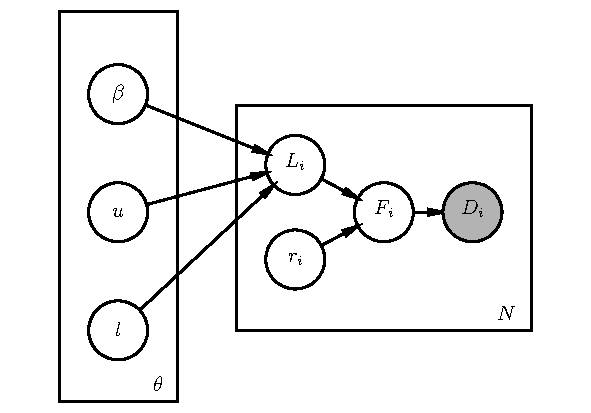
\includegraphics{fig/prob_graph_model}
\end{center}
\caption{The hierarchical model to generate random samples of galaxies. Luminosity depends on the population parameters $\theta = (\beta, l, u)$. The real flux is computed directly from the real luminosity and the distance. Observational statistical error only affects the flux measurement and the noise depends on the real flux only. The selection effect $p(D_i < T) = 0$ is not indicated on the graph.}
\label{fig:model}
\end{figure}

\begin{figure}
\begin{center}
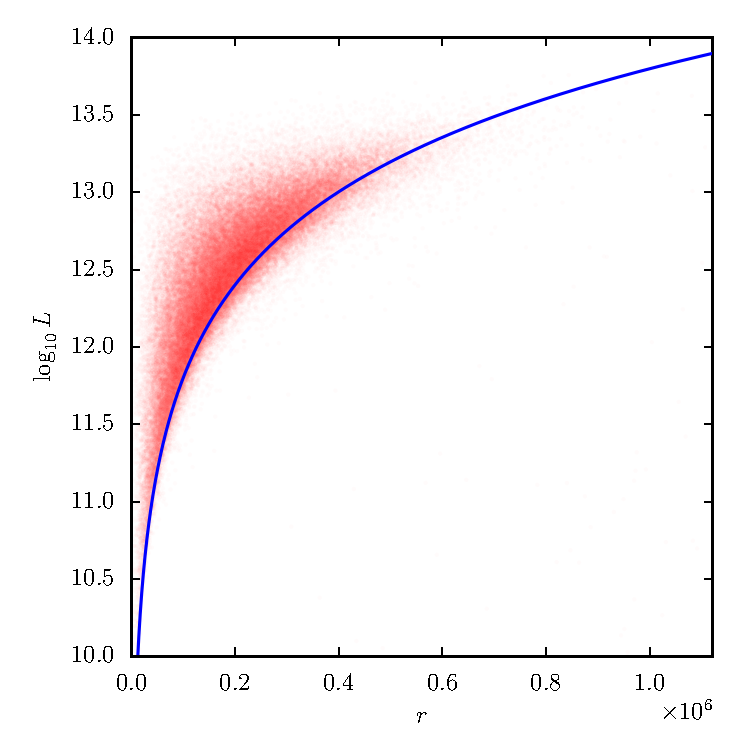
\includegraphics{{fig/lum_vs_dist}}
\end{center}
\caption{A random sample of luminosities generated using our model, plotted as a function of distance. Red dots mark individual object, whereas the blue curve represent the luminosity equivalent of the flux limit $T = 5.0$. Since the flux limit is applied to the noisy fluxes, a significant fraction of the objects is scattered below the luminosity limit. Any parameter estimation method has to account for this effect in order to successfully approximate the population parameters.}
\label{fig:lum_vs_dist}
\end{figure}

